\chapter{Sviluppo software agile}
Le aziende operano ora in un ambiente globale in rapido cambiamento. Il software è parte di quasi tutte le operazioni aziendali, quindi il nuovo software deve essere sviluppato rapidamente per cogliere le nuove opportunità e rispondere alla pressione competitiva. Lo sviluppo e la consegna rapida del software sono quindi i requisiti più critici per la maggior parte dei sistemi aziendali.

I processi di sviluppo software plan-driven, che specificano completamente i requisiti e poi progettano, costruiscono e testano un sistema, non sono adatti allo sviluppo rapido del software. Man mano che i requisiti cambiano o emergono problemi nei requisiti, il design o l'implementazione del sistema devono essere rielaborati e ritestati.

Lo sviluppo rapido del software ha veramente preso piede alla fine degli anni '90 con lo sviluppo dell'idea di "metodi agili" progettati per produrre software utile in tempi rapidi. Tutti i metodi agili proposti condividono una serie di caratteristiche comuni:
\begin{enumerate}
    \item I processi di specifica, progettazione e implementazione sono intrecciati.
    \item Il sistema viene sviluppato in una serie di incrementi. Gli utenti finali e altri stakeholder del sistema sono coinvolti nella specifica e valutazione di ciascun incremento.
    \item Viene utilizzato un ampio supporto di strumenti per sostenere il processo di sviluppo.
    \item Non esiste una specifica dettagliata del sistema, e la documentazione di progettazione è ridotta al minimo o generata automaticamente.
\end{enumerate}
Gli approcci agili allo sviluppo software considerano la progettazione e l'implementazione come le attività centrali nel processo software. Includono altre attività, come l'elicitazione dei requisiti e il testing, nella progettazione e nell'implementazione. Al contrario, un approccio plan-driven per l'ingegneria del software identifica fasi separate nel processo software, con output associati a ciascuna fase. Gli output di una fase vengono utilizzati come base per pianificare l'attività di processo successiva.

La Figura \ref{fig:plan-driven-agile-development} mostra le distinzioni essenziali tra approcci plan-driven e approcci agili alla specifica del sistema. 

\begin{figure}[ht]
    \centering
    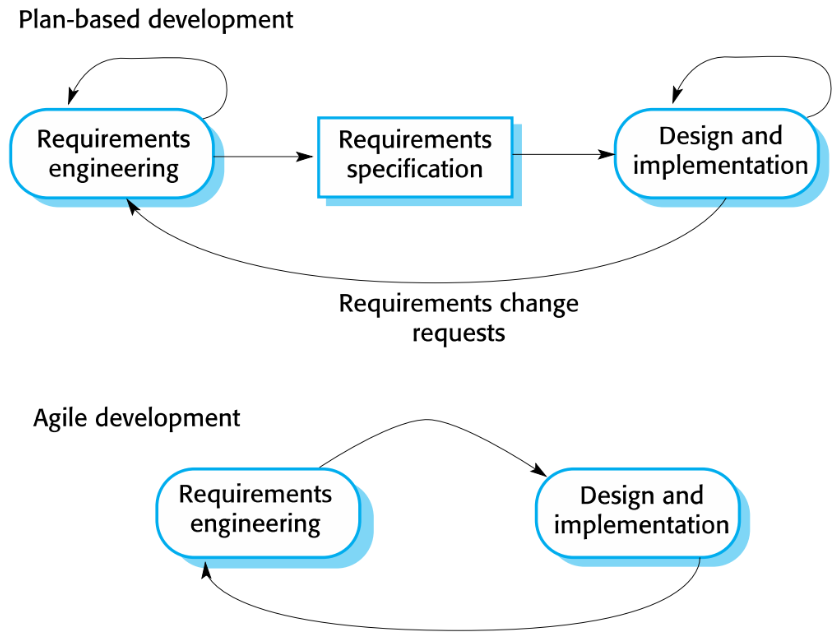
\includegraphics[width=0.55\linewidth]{images/plan-driven-agile-development.PNG}
    \caption{Sviluppo plan-driven e agile}
    \label{fig:plan-driven-agile-development}
\end{figure}

\section{Metodi agili}
Negli anni '80 e nei primi anni '90, era diffusa l'idea che il modo migliore per ottenere un software migliore fosse attraverso un'attenta pianificazione del progetto. L'insoddisfazione per questi approcci pesanti all'ingegneria del software ha portato allo sviluppo di metodi agili alla fine degli anni '90. Questi metodi hanno permesso ai team di sviluppo di concentrarsi sul software stesso piuttosto che sulla sua progettazione e documentazione. Sono più adatti allo sviluppo di applicazioni in cui i requisiti del sistema di solito cambiano rapidamente durante il processo di sviluppo. Sono progettati per consegnare software funzionante rapidamente ai clienti, che possono poi proporre nuovi requisiti e cambiamenti da includere nelle iterazioni successive del sistema. L'obiettivo è ridurre le spese generali nel processo software ed eliminando documentazione che probabilmente non verrà mai utilizzata.

La filosofia dietro i metodi agili si riflette nel manifesto agile pubblicato dai principali sviluppatori di questi metodi. Questo manifesto afferma:

\begin{center}
\begin{minipage}{0.9\textwidth}
\textit{Siamo alla scoperta di modi migliori per sviluppare software facendolo e aiutando altri a farlo. Attraverso questo lavoro, abbiamo imparato a dare valore a:}

\textit{Le persone e le interazioni più che i processi e gli strumenti}

\textit{Il software funzionante più che la documentazione esaustiva}

\textit{La collaborazione con il cliente più che la negoziazione del contratto}

\textit{Rispondere ai cambiamenti più che seguire un piano}

\textit{Vale a dire, mentre c'è valore negli elementi a destra, diamo più valore agli elementi a sinistra.}
\end{minipage}
\end{center}
Tutti i metodi agili suggeriscono che il software debba essere sviluppato e consegnato in modo incrementale. Questi metodi si basano su diversi processi agili, ma condividono un insieme di principi, basati sul manifesto agile, e quindi hanno molto in comune (vedi Tabella \ref{tab:principi-metodi-agili}).

\begin{table}[ht]
\centering
\rowcolors{2}{lightblue}{lightgray}
\begin{tabular}{|p{5cm}|p{10cm}|}
\hline
\rowcolor{headerblue}
\textbf{\textcolor{white}{Principio}} & \textbf{\textcolor{white}{Descrizione}} \\
\hline
Coinvolgimento del cliente & I clienti dovrebbero essere coinvolti strettamente durante tutto il processo di sviluppo. Il loro ruolo è fornire e prioritizzare i nuovi requisiti del sistema e valutare le iterazioni del sistema. \\
\hline
Consegna incrementale & Il software viene sviluppato in incrementi, con il cliente che specifica i requisiti da includere in ogni incremento. \\
\hline
Persone, non processi & Le competenze del team di sviluppo dovrebbero essere riconosciute e sfruttate. I membri del team dovrebbero essere lasciati liberi di sviluppare i propri modi di lavorare senza processi prescrittivi. \\
\hline
Accogliere il cambiamento & È necessario aspettarsi che i requisiti del sistema cambino e progettare il sistema per adattarsi a questi cambiamenti. \\
\hline
Mantenere la semplicità & Concentrarsi sulla semplicità sia nel software che viene sviluppato, sia nel processo di sviluppo. Ovunque sia possibile, lavorare attivamente per eliminare la complessità dal sistema. \\
\hline
\end{tabular}
\caption{I principi dei metodi agili}
\label{tab:principi-metodi-agili}
\end{table}

I metodi agili hanno avuto particolare successo in due tipi di sviluppo di sistemi:
\begin{enumerate}
    \item Sviluppo di prodotti, in cui un'azienda di software sviluppa un prodotto di piccole o medie dimensioni per la vendita. Praticamente tutti i prodotti software e le app vengono ora sviluppati utilizzando un approccio agile.
    \item Sviluppo di sistemi personalizzati all'interno di un'organizzazione, dove c'è un chiaro impegno da parte del cliente a essere coinvolto nel processo di sviluppo e dove ci sono pochi stakeholder esterni e regolamenti che influenzano il software.
\end{enumerate}

\section{Tecniche di sviluppo agili}
Le idee alla base dei metodi agili sono state sviluppate all'incirca nello stesso periodo da diverse persone negli anni '90. Tuttavia, l'approccio che probabilmente ha avuto il maggiore impatto nel cambiare la cultura dello sviluppo software è stato lo sviluppo di Extreme Programming (XP). Il termine è stato coniato da Kent Beck (Beck 1998) poiché l'approccio è stato sviluppato portando a livelli "estremi" le pratiche riconosciute come buone, come lo sviluppo iterativo. Ad esempio, in XP, diverse nuove versioni di un sistema possono essere sviluppate da diversi programmatori, integrate e testate in un solo giorno. La Figura \ref{fig:extreme-programming-release-cycle} illustra il processo XP per produrre un incremento del sistema in fase di sviluppo.

\begin{figure}[ht]
    \centering
    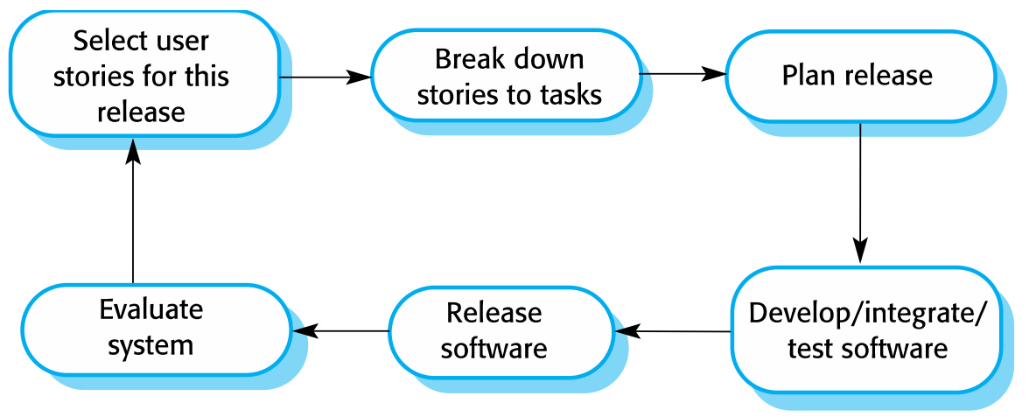
\includegraphics[width=0.6\linewidth]{images/extreme-programming-release-cycle.PNG}
    \caption{Il ciclo di rilascio dell'extreme programming}
    \label{fig:extreme-programming-release-cycle}
\end{figure}

Extreme Programming è stato controverso poiché ha introdotto una serie di pratiche agili che erano piuttosto diverse dalle pratiche di sviluppo di quel tempo. Queste pratiche sono riassunte nella Tabella \ref{tab:principi-pratiche-extreme-programming} e riflettono i principi del manifesto agile:

\begin{table}[ht]
\centering
\rowcolors{2}{lightblue}{lightgray}
\begin{tabular}{|p{5cm}|p{10cm}|}
\hline
\rowcolor{headerblue}
\textbf{\textcolor{white}{Principio o pratica}} & \textbf{\textcolor{white}{Descrizione}} \\
\hline
Pianificazione incrementale & I requisiti sono registrati su "carte delle storie" e le storie da includere in un rilascio sono determinate in base al tempo disponibile e alla loro priorità relativa. Gli sviluppatori suddividono queste storie in "compiti" di sviluppo.
\\\hline Piccoli rilasci & Il set minimo di funzionalità utile che fornisce valore aziendale viene sviluppato per primo. I rilasci del sistema sono frequenti e aggiungono funzionalità in modo incrementale al primo rilascio.
\\\hline Progettazione semplice & Viene effettuata solo la progettazione necessaria per soddisfare i requisiti attuali e non di più.
\\\hline Sviluppo test-first & Un framework di test unitario automatizzato viene utilizzato per scrivere test per una nuova funzionalità prima che la funzionalità stessa venga implementata.
\\\hline Refactoring & Tutti gli sviluppatori sono tenuti a rifattorizzare continuamente il codice non appena vengono trovati potenziali miglioramenti. Questo mantiene il codice semplice e manutenibile.
\\\hline Programmazione in coppia & Gli sviluppatori lavorano in coppia, controllando reciprocamente il lavoro e fornendo supporto per svolgere sempre un buon lavoro.
\\\hline Proprietà collettiva & Le coppie di sviluppatori lavorano su tutte le aree del sistema, in modo che non si sviluppino isole di competenza e tutti gli sviluppatori si assumano la responsabilità per tutto il codice. Chiunque può modificare qualsiasi parte.
\\\hline Integrazione continua & Non appena un compito è completato, viene integrato nel sistema completo. Dopo ogni integrazione, tutti i test unitari del sistema devono passare.
\\\hline Ritmo sostenibile & Lavorare molte ore di straordinario non è accettabile, poiché spesso l'effetto netto è una riduzione della qualità del codice e della produttività a medio termine.
\\\hline Cliente in loco & Un rappresentante dell'utente finale del sistema (il Cliente) deve essere disponibile a tempo pieno per il team XP. In un processo di extreme programming, il cliente è membro del team di sviluppo ed è responsabile di portare i requisiti del sistema al team per l'implementazione.
\\\hline 
\end{tabular}
\caption{Principi e pratiche di extreme programming}
\label{tab:principi-pratiche-extreme-programming}
\end{table}

\begin{enumerate}
    \item Sviluppo incrementale è supportato attraverso piccoli e frequenti rilasci del sistema.
    \item Coinvolgimento del cliente è supportato attraverso il continuo coinvolgimento del cliente nel team di sviluppo.
    \item Persone, non processi sono supportate attraverso la programmazione in coppia, la proprietà collettiva del codice del sistema e un processo di sviluppo sostenibile che non prevede lunghe ore di lavoro.
    \item Il cambiamento viene accolto attraverso i rilasci regolari del sistema ai clienti.
    \item Mantenere la semplicità è supportato da un refactoring costante che migliora la qualità del codice.
\end{enumerate}
In pratica, l'applicazione di Extreme Programming come originariamente proposto si è rivelata più difficile del previsto. Non può essere facilmente integrato con le pratiche di gestione della maggior parte delle aziende. Pertanto, le aziende che adottano metodi agili scelgono le pratiche XP che sono più adatte al loro modo di lavorare. A volte queste sono incorporate nei loro processi di sviluppo, ma più comunemente vengono utilizzate in combinazione con un metodo agile più focalizzato sulla gestione.

\subsection{Storie degli utenti}
I requisiti software cambiano costantemente. Per gestire questi cambiamenti, i metodi agili prevedono l'idea delle "storie degli utenti," dove una storia utente è uno scenario d'uso che potrebbe essere vissuto da un utilizzatore del sistema.

Per quanto possibile, il cliente del sistema lavora a stretto contatto con il team di sviluppo e discute questi scenari con gli altri membri del team. Insieme, sviluppano una "carta della storia" che descrive brevemente una storia che incapsula le esigenze del cliente.

Le storie degli utenti possono essere utilizzate nella pianificazione delle iterazioni del sistema. Una volta sviluppate le carte delle storie, il team di sviluppo le suddivide in compiti e stima lo sforzo e le risorse necessari per implementare ciascun compito. Il cliente poi assegna la priorità alle storie da implementare, scegliendo quelle che possono essere utilizzate immediatamente per fornire supporto operativo.

\begin{Example}{Una storia di “prescrizione di farmaci”}{}
Il record del paziente deve essere aperto per l'inserimento. Fare clic sul campo relativo ai farmaci e selezionare 'medicazione corrente', 'nuova medicazione' o 'formulario'.
\begin{itemize}
    \item Se si seleziona 'medicazione corrente', verrà richiesto di controllare il dosaggio. Se si desidera cambiarlo, inserire il nuovo dosaggio e confermare la prescrizione.
    \item Se si sceglie 'nuova medicazione', il sistema presuppone che si sappia quale farmaco prescrivere. Digitare le prime lettere del nome del farmaco e verrà visualizzato un elenco di farmaci possibili. Selezionare il farmaco richiesto, verificare che il farmaco scelto sia corretto, inserire il dosaggio e confermare la prescrizione.
    \item Se si sceglie 'formulario', verrà visualizzata una casella di ricerca per cercare nel formulario approvato. Selezionare il farmaco richiesto, verificare che sia corretto, inserire il dosaggio e confermare la prescrizione.
\end{itemize}
In tutti i casi, il sistema controllerà che il dosaggio sia all'interno del range approvato e chiederà di modificarlo se è fuori dal range raccomandato.

Dopo aver confermato la prescrizione, verrà visualizzata per un controllo finale. Fare clic su 'OK' per registrare la prescrizione nel database di audit oppure su 'Modifica' per rientrare nel processo di prescrizione.

\begin{minipage}{\textwidth}
    \centering
    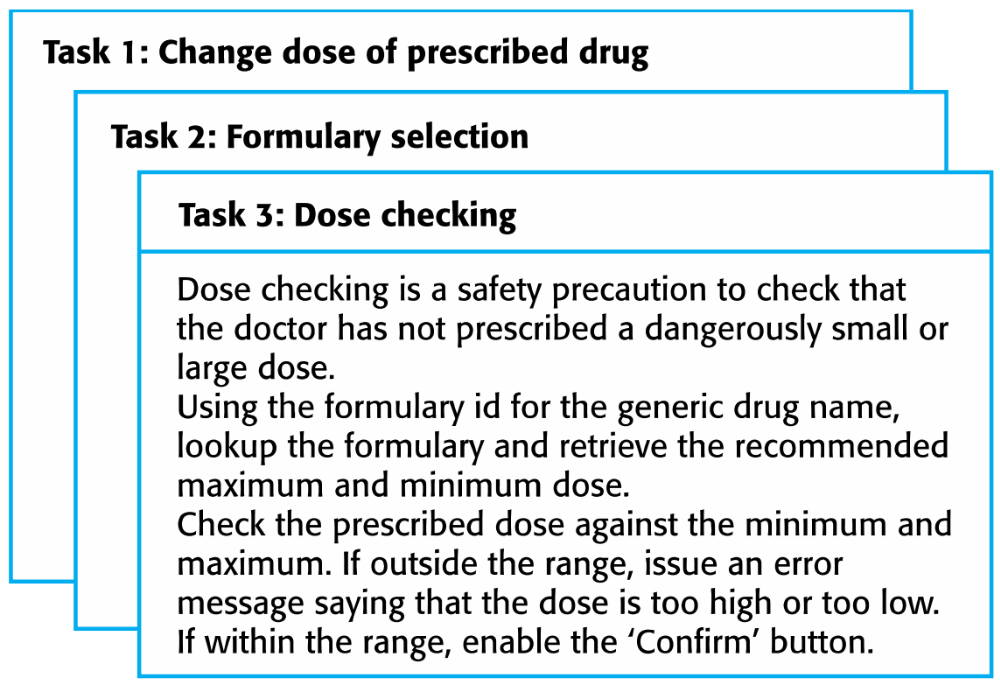
\includegraphics[width=0.6\textwidth]{images/es-task-card.PNG}
    %\captionof{figure}{}
\end{minipage}
\end{Example}

\subsection{Refactoring}
Un concetto fondamentale nell'ingegneria del software tradizionale è progettare per il cambiamento, ossia prevedere le modifiche future al software e progettarlo in modo che possano essere facilmente implementate. Tuttavia, l'Extreme Programming (XP) ha abbandonato questo principio, sostenendo che spesso progettare per il cambiamento è uno spreco di tempo. Le modifiche anticipate spesso non si materializzano o si verificano richieste di cambiamento completamente diverse.

XP propone invece che il codice in sviluppo venga continuamente rifattorizzato. Il refactoring consiste nel cercare miglioramenti possibili al software e implementarli immediatamente, anche in assenza di una necessità immediata. Se i membri del team individuano codice migliorabile, apportano queste modifiche per evitare che, col tempo, la struttura del software si degradi.

Esempi di refactoring includono la riorganizzazione di gerarchie di classi per eliminare codice duplicato, la pulizia e rinominazione di attributi e metodi, e la sostituzione di sezioni di codice simili con chiamate a metodi definiti in una libreria.

\subsection{Test-first development}
L’Extreme Programming (XP) ha sviluppato un nuovo approccio al test del software per affrontare le difficoltà di test senza una specifica formale. I test sono automatizzati e centrali nel processo di sviluppo: lo sviluppo non può procedere finché tutti i test non sono stati eseguiti con successo. Le caratteristiche principali del testing in XP sono:
\begin{enumerate}
    \item Sviluppo con test preliminari,
    \item Sviluppo incrementale dei test a partire da scenari,
    \item Coinvolgimento dell'utente nello sviluppo e nella validazione dei test,
    \item Utilizzo di framework di testing automatizzato per eseguire tutti i test dei componenti ogni volta che viene creata una nuova versione.
\end{enumerate}
Invece di scrivere il codice e successivamente i test, i test vengono scritti prima del codice. Questo consente di eseguire i test durante la scrittura del codice e scoprire eventuali problemi immediatamente.

Nel test-first development, gli sviluppatori devono comprendere a fondo la specifica per poter scrivere i test. Ciò significa che eventuali ambiguità e omissioni devono essere chiarite prima che inizi l’implementazione.

\begin{Example}{Verifica della dose}{}
\textit{Input:}
\begin{enumerate}
    \item Un numero in mg che rappresenta una singola dose del farmaco.
    \item Un numero che rappresenta il numero di dosi giornaliere.
\end{enumerate}
\textit{Tests:}
\begin{enumerate}
    \item Test per singola dose corretta, ma frequenza troppo alta.
    \item Test per dose singola troppo alta o troppo bassa.
    \item Test per frequenza della dose troppo alta o troppo bassa.
    \item Test per dose e frequenza all'interno del range consentito.
\end{enumerate}
\textit{Output:} Se i valori inseriti sono corretti, restituisce OK. In caso contrario, restituisce un messaggio di errore che specifica se la dose o la frequenza è fuori dal range sicuro.
\end{Example} 

L’automazione del testing è essenziale per lo sviluppo con test preliminari. I test sono scritti come componenti eseguibili prima dell'implementazione del task. Questi componenti dovrebbero essere autonomi, simulare l'invio di input da testare e verificare che il risultato soddisfi la specifica dell'output. Un esempio comune di framework di testing automatizzato è JUnit, utilizzato per testare programmi Java.

Nonostante i vantaggi di questo approccio, ci sono problemi nel garantire la completezza della copertura dei test:
\begin{enumerate}
    \item Gli sviluppatori spesso preferiscono programmare piuttosto che scrivere test, e talvolta prendono scorciatoie scrivendo test incompleti.
    \item Alcuni test sono difficili da scrivere in modo incrementale, come quelli per le interfacce utente complesse.
\end{enumerate}
Pertanto, anche un ampio set di test eseguiti frequentemente potrebbe non garantire la copertura completa del sistema, e bug non rilevati potrebbero comunque essere presenti nelle versioni rilasciate.

\subsection{Pair programming}
Un'altra pratica innovativa introdotta in XP è che i programmatori lavorano in coppia per sviluppare il software. La coppia di programmatori si siede allo stesso computer per sviluppare il software. Tuttavia, la stessa coppia non programma sempre insieme. Piuttosto, le coppie vengono formate dinamicamente in modo che tutti i membri del team lavorino con ciascuno degli altri durante il processo di sviluppo.

La programmazione in coppia ha una serie di vantaggi:
\begin{enumerate}
    \item Supporta l'idea di proprietà e responsabilità collettiva del sistema.
    \item Funziona come un processo di revisione informale perché ogni riga di codice è esaminata da almeno due persone.
    \item Incoraggia il refactoring per migliorare la struttura del software.
\end{enumerate}
La condivisione delle conoscenze che avviene durante la programmazione in coppia è molto importante in quanto riduce i rischi complessivi per un progetto quando i membri del team se ne vanno. La programmazione in coppia non è necessariamente inefficiente e ci sono alcune prove che suggeriscono che una coppia che lavora insieme è più efficiente di due programmatori che lavorano separatamente.

\section{Gestione agile dei progetti}
In qualsiasi attività legata al software, i manager devono sapere cosa sta succedendo e se un progetto è in grado di raggiungere i suoi obiettivi e consegnare il software in tempo e con il budget previsto. Gli approcci alla sviluppo software plan driven si sono evoluti per soddisfare questa necessità: i manager redigono un piano per il progetto che mostra cosa dovrebbe essere consegnato, quando dovrebbe essere consegnato e chi lavorerà allo sviluppo dei deliverable del progetto. Un approccio basato su piani richiede che un manager abbia una visione stabile di tutto ciò che deve essere sviluppato e dei processi di sviluppo.

Scrum è un metodo agile che si concentra sulla gestione dello sviluppo iterativo piuttosto che su pratiche agili specifiche. Ci sono tre fasi in Scrum:
\begin{enumerate}
    \item La fase iniziale è una fase di pianificazione generale in cui si stabiliscono gli obiettivi generali per il progetto e si progetta l'architettura software.
    \item Questa è seguita da una serie di cicli di sprint, in cui ogni ciclo sviluppa un incremento del sistema.
    \item La fase di chiusura del progetto conclude il progetto, completa la documentazione richiesta come frame di aiuto del sistema e manuali utente e valuta le lezioni apprese dal progetto.
\end{enumerate}

\begin{table}[ht]
\centering
\rowcolors{2}{lightblue}{lightgray}
\begin{tabular}{|p{4cm}|p{11cm}|}
\hline
\rowcolor{headerblue}
\textbf{\textcolor{white}{Termine Scrum}} & \textbf{\textcolor{white}{Definizione}} \\\hline
Team di sviluppo & Un gruppo auto-organizzato di sviluppatori software, composto da non più di sette persone. Sono responsabili dello sviluppo del software e dei documenti essenziali.
\\\hline
Incremento di prodotto potenzialmente rilasciabile & L'incremento software consegnato alla fine di uno sprint, che dovrebbe essere in uno stato "potenzialmente rilasciabile", senza bisogno di ulteriori lavori come test. In pratica, non sempre è raggiungibile.
\\\hline
Backlog del prodotto & Una lista di attività o elementi "da fare" che il team Scrum deve affrontare. Possono essere definizioni di funzionalità del software, requisiti, user stories o compiti supplementari come la definizione dell'architettura o la documentazione utente.
\\\hline
Proprietario del prodotto & Una persona (o un piccolo gruppo) incaricata di identificare le funzionalità o i requisiti del prodotto, priorizzarli per lo sviluppo e rivedere continuamente il backlog per garantire che il progetto continui a soddisfare i bisogni critici del business. Il Product Owner può essere un cliente o un product manager di un'azienda di software o un altro rappresentante degli stakeholder.
\\\hline
Scrum & Un incontro giornaliero del team Scrum per rivedere i progressi e dare priorità al lavoro da fare durante il giorno. Idealmente, dovrebbe essere un breve incontro faccia a faccia con l'intero team.
\\\hline
ScrumMaster & Lo ScrumMaster è responsabile di assicurare che il processo Scrum venga seguito e guida il team nell'uso efficace di Scrum. È responsabile dell'interfaccia con il resto dell'azienda e di garantire che il team Scrum non venga distratto da interferenze esterne. I creatori di Scrum sottolineano che lo ScrumMaster non dovrebbe essere considerato un project manager, anche se potrebbe non essere facile vedere la differenza.
\\\hline
Sprint & Una iterazione di sviluppo, generalmente di durata compresa tra 2 e 4 settimane.
\\\hline
Velocità & Una stima di quanto backlog il team può affrontare in un singolo sprint. Comprendere la velocità del team aiuta a stimare cosa si può coprire in uno sprint e a misurare le performance.
\\\hline
\end{tabular}
\caption{Terminologia Scrum}
\label{tab:terminologia-scrum}
\end{table}

\begin{figure}[ht]
    \centering
    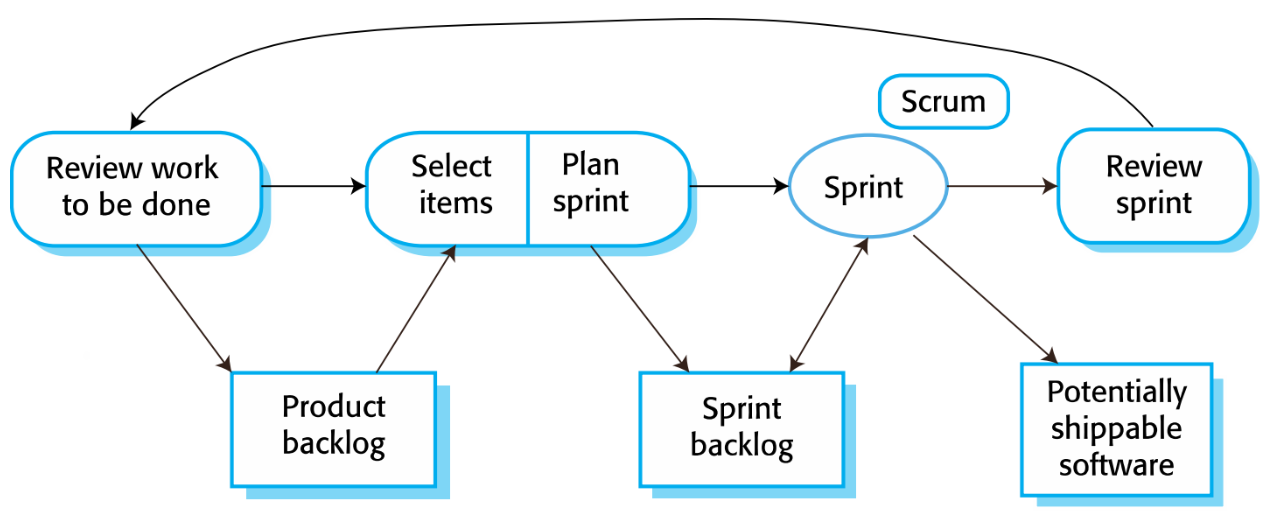
\includegraphics[width=0.6\linewidth]{images/scrum-sprint-cycle.PNG}
    \caption{Ciclo sprint Scrum}
    \label{fig:scrum-sprint-cycle}
\end{figure}

Ogni ciclo sprint dura un periodo di tempo fisso, solitamente tra le 2 e le 4 settimane. Il punto di partenza per la pianificazione è il product backlog, ovvero l'elenco del lavoro da svolgere sul progetto. La fase di selezione coinvolge tutto il team di progetto che lavora con il cliente per selezionare le caratteristiche e le funzionalità dal product backlog da sviluppare durante lo sprint.

Una volta concordati, il team si organizza per sviluppare il software. Durante questa fase il team è isolato dal cliente e dall'organizzazione, con tutte le comunicazioni incanalate attraverso il cosiddetto "Scrum master". Il ruolo dello Scrum master è quello di proteggere il team di sviluppo da distrazioni esterne. Alla fine dello sprint, il lavoro svolto viene rivisto e presentato alle parti interessate. Quindi inizia il ciclo di sprint successivo.
Lo "Scrum master" è un facilitatore che organizza riunioni giornaliere, tiene traccia dell'arretrato di lavoro da svolgere, registra le decisioni, misura i progressi rispetto all'arretrato e comunica con i clienti e la dirigenza esterna al team. 

L'intero team partecipa a brevi riunioni giornaliere (Scrum) in cui tutti i membri del team condividono informazioni, descrivono i progressi dall'ultima riunione, i problemi emersi e cosa è previsto per il giorno successivo. Ciò significa che tutti nel team sanno cosa sta succedendo e, se si presentano problemi, possono riprogrammare il lavoro a breve termine per affrontarli.

I benefici del metodo Scrum sono:
\begin{enumerate}
    \item Il prodotto è suddiviso in una serie di componenti gestibili e comprensibili a cui gli stakeholder possono rapportarsi.
    \item I requisiti instabili non bloccano i progressi.
    \item L'intero team ha visibilità su tutto e, di conseguenza, la comunicazione del team e il morale migliorano.
    \item I clienti vedono la consegna puntuale degli incrementi e ricevono feedback su come funziona il prodotto.
    \item Si crea fiducia tra i clienti e gli sviluppatori, e si instaura una cultura positiva in cui tutti si aspettano che il progetto abbia successo.
\end{enumerate}
Tuttavia, gran parte dello sviluppo software ora coinvolge team distribuiti, con membri del team situati in luoghi diversi in tutto il mondo. Di conseguenza, ci sono stati sviluppi di Scrum per ambienti di sviluppo distribuiti e per il lavoro multi-team (vedi Figura \ref{fig:distributed-scrum}).

\begin{figure}[ht]
    \centering
    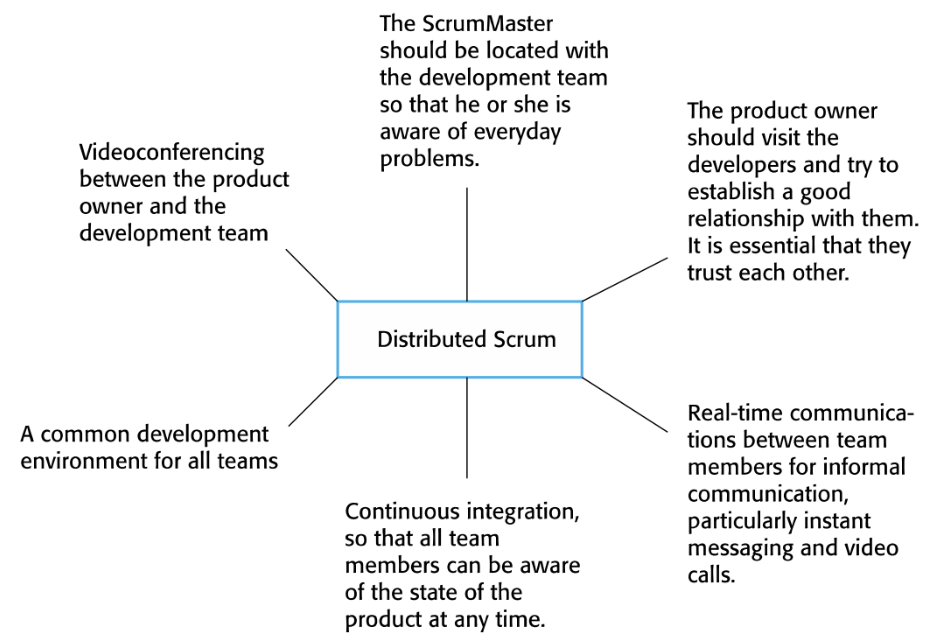
\includegraphics[width=0.6\linewidth]{images/distributed-scrum.PNG}
    \caption{Scrum distribuito}
    \label{fig:distributed-scrum}
\end{figure}

\section{Scalabilità dei metodi agili}
I metodi agili hanno dimostrato di essere efficaci per progetti di piccole e medie dimensioni che possono essere sviluppati da un piccolo team co-localizzato. A volte si sostiene che il successo di questi metodi derivi dal miglioramento delle comunicazioni che è possibile quando tutti lavorano insieme. Naturalmente, la necessità di una consegna più rapida del software, che si adatta meglio alle esigenze dei clienti, si applica anche a sistemi di grandi dimensioni e a grandi aziende.

La scalabilità dei metodi agili ha aspetti strettamente correlati:
\begin{enumerate}
    \item "Scaling up" riguarda l'uso di metodi agili per sviluppare grandi sistemi software che non possono essere sviluppati da un piccolo team.
    \item "Scaling out" riguarda il modo in cui i metodi agili possono essere introdotti in una grande organizzazione con molti anni di esperienza nello sviluppo software.
\end{enumerate}

\subsection{Problemi pratici con i metodi agili}
Per i sistemi grandi e di lunga durata sviluppati da un'azienda software per un cliente esterno, l'uso di un approccio agile presenta una serie di problemi.
\begin{enumerate}
    \item L'informalità dello sviluppo agile è incompatibile con l'approccio legale alla definizione dei contratti comunemente utilizzato nelle grandi aziende.
    \item I metodi agili sono più appropriati per lo sviluppo di nuovo software piuttosto che per la manutenzione del software. Tuttavia, la maggior parte dei costi software nelle grandi aziende proviene dalla manutenzione dei loro sistemi software esistenti.
    \item I metodi agili sono progettati per piccoli team co-localizzati, ma gran parte dello sviluppo software ora coinvolge team distribuiti a livello mondiale.
\end{enumerate}
Le questioni contrattuali possono essere un grosso problema quando si utilizzano metodi agili. Quando il cliente del sistema utilizza un'organizzazione esterna per lo sviluppo del sistema, viene redatto un contratto per lo sviluppo software tra loro. Poiché lo sviluppo intrecciato di requisiti e codice è fondamentale per i metodi agili, non esiste una dichiarazione definitiva dei requisiti che possa essere inclusa nel contratto. Di conseguenza, i metodi agili devono fare affidamento su contratti in cui il cliente paga per il tempo richiesto per lo sviluppo del sistema piuttosto che per lo sviluppo di un insieme specifico di requisiti.

Una grande quantità di sforzi di ingegneria del software viene dedicata alla manutenzione e all'evoluzione dei sistemi software esistenti. Quindi, se i metodi agili devono avere successo, devono supportare la manutenzione così come lo sviluppo originale.

Possono sorgere tre tipi di problemi:
\begin{itemize}
    \item Mancanza di documentazione del prodotto.
    \item Mantenere i clienti coinvolti nel processo di sviluppo.
    \item Mantenere la continuità del team di sviluppo.
\end{itemize}

\subsection{Metodi agili e metodi plan-driven}
Un requisito fondamentale per scalare i metodi agili è integrarli con approcci basati sulla pianificazione. Per decidere il bilanciamento tra un approccio plan-driven e uno agile, è necessario rispondere a una serie di domande:
\begin{enumerate}
    \item È importante avere una specifica e una progettazione molto dettagliate prima di passare all'implementazione, forse per motivi contrattuali? Se sì, probabilmente è necessario utilizzare un approccio plan-driven.
    \item È realistica una strategia di consegna incrementale, in cui si consegna il software ai clienti o ad altri portatori di interesse del sistema e si ottiene un feedback rapido da loro? In tal caso, puoi considerare l'utilizzo di metodi agili.
    \item Quanto è grande il sistema che si sta sviluppando? I metodi agili sono più efficaci quando il sistema può essere sviluppato con un piccolo team co-localizzato che può comunicare in modo informale. Questo potrebbe non essere possibile per sistemi di grandi dimensioni che richiedono team di sviluppo più grandi, quindi potrebbe essere necessario utilizzare un approccio plan-driven.
\end{enumerate}

\begin{table}[ht]
\centering
\rowcolors{2}{lightblue}{lightgray}
\begin{tabular}{|p{4cm}|p{11cm}|}
\hline
\rowcolor{headerblue}
\textbf{\textcolor{white}{Principio}} & \textbf{\textcolor{white}{Pratica}} \\\hline
Coinvolgimento del cliente & Questo dipende dall'avere un cliente che sia disposto e in grado di trascorrere del tempo con il team di sviluppo e che possa rappresentare tutti gli stakeholder del sistema. Spesso, i rappresentanti dei clienti hanno altre richieste sul loro tempo e non possono partecipare pienamente allo sviluppo del software. Quando ci sono stakeholder esterni, come i regolatori, è difficile rappresentare le loro opinioni al team agile.\\\hline
Accogliere il cambiamento & Dare priorità ai cambiamenti può essere estremamente difficile, specialmente in sistemi con molti stakeholder. Tipicamente, ogni stakeholder attribuisce priorità diverse a cambiamenti differenti.\\\hline
Consegna incrementale & Iterazioni rapide e pianificazione a breve termine per lo sviluppo non si adattano sempre ai cicli di pianificazione a lungo termine della pianificazione aziendale e del marketing. I responsabili marketing potrebbero aver bisogno di conoscere le caratteristiche del prodotto diversi mesi in anticipo per preparare una campagna di marketing efficace.\\\hline
Mantenere la semplicità & Sotto pressione dai programmi di consegna, i membri del team potrebbero non avere tempo per attuare semplificazioni desiderabili del sistema.\\\hline
Persone, non processi & I singoli membri del team potrebbero non avere personalità adatte per il coinvolgimento intenso che è tipico dei metodi agili e, pertanto, potrebbero non interagire bene con gli altri membri del team.
\\\hline
\end{tabular}
\caption{Principi agili e pratica organizzativa}
\label{tab:agile-principles}
\end{table}

\begin{figure}[ht]
    \centering
    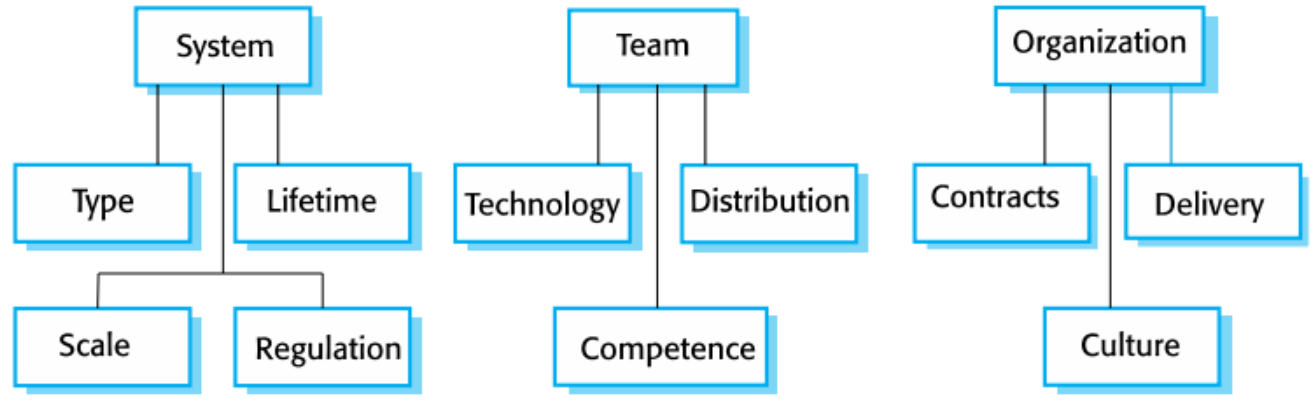
\includegraphics[width=0.7\linewidth]{images/agile-plan-based-factors.PNG}
    \caption{Fattori agili e plan-based}
    \label{fig:agile-plan-based-factors}
\end{figure}

È necessario fare una certa pianificazione, progettazione e documentazione iniziali nel processo di ingegneria dei sistemi. Alcuni dei problemi chiave sono i seguenti:
\begin{enumerate}
    \item Quanto è grande il sistema che si sta sviluppando? I metodi agili sono più efficaci quando il sistema può essere sviluppato con un team relativamente piccolo e co-locato che può comunicare informalmente.
    \item Che tipo di sistema si sta sviluppando? I sistemi che richiedono molte analisi prima dell'implementazione di solito necessitano di una progettazione abbastanza dettagliata per svolgere questa analisi.
    \item Qual è la durata prevista del sistema? I sistemi di lunga durata potrebbero richiedere più documentazione di progettazione per comunicare le intenzioni originali degli sviluppatori del sistema al team di supporto.
    \item Il sistema è soggetto a regolamentazione esterna? Se un sistema deve essere approvato da un regolatore esterno allora probabilmente sarà necessario produrre documentazione dettagliata come parte del caso di sicurezza del sistema.
    \item Qual è il livello di competenza dei progettisti e dei programmatori nel team di sviluppo? A volte si sostiene che i metodi agili richiedano livelli di competenza più elevati rispetto agli approcci basati sulla pianificazione in cui i programmatori traducono semplicemente un design dettagliato in codice.
    \item Come è organizzato il team di sviluppo? Se il team di sviluppo è distribuito potrebbe essere necessario sviluppare documenti di progettazione per comunicare tra i team di sviluppo.
    \item Quali tecnologie sono disponibili per supportare lo sviluppo del sistema? Se stai sviluppando un sistema utilizzando un IDE che non ha buoni strumenti per la visualizzazione e l'analisi del codice, allora potrebbe essere necessaria più documentazione di progettazione.
\end{enumerate}

\subsection{Metodi agili per grandi sistemi}
I metodi agili devono evolversi per essere utilizzati nello sviluppo software su larga scala. La ragione fondamentale di ciò è che i sistemi software di grande scala sono molto più complessi e difficili da comprendere e gestire rispetto ai sistemi o ai prodotti software di piccola scala. Sei fattori principali contribuiscono a questa complessità:
\begin{enumerate}
    \item \textit{Sistemi di sistemi:} I grandi sistemi sono solitamente sistemi di sistemi, collezioni di sistemi separati che comunicano tra loro, dove team separati sviluppano ciascun sistema. Spesso, questi team lavorano in luoghi diversi, a volte in fusi orari diversi.
    \item \textit{Sistemi brownfield:} I grandi sistemi sono sistemi brownfield; cioè, includono e interagiscono con diversi sistemi esistenti. Molti dei requisiti del sistema riguardano questa interazione e quindi non si prestano realmente alla flessibilità e allo sviluppo incrementale.
    \item \textit{Configurazione del sistema:} Dove diversi sistemi sono integrati per creare un sistema, una frazione significativa dello sviluppo è dedicata alla configurazione del sistema piuttosto che allo sviluppo di codice originale.
    \item \textit{Regole e normative esterne:} I grandi sistemi e i loro processi di sviluppo sono spesso vincolati da regole e normative esterne che limitano il modo in cui possono essere sviluppati.
    \item \textit{Lungo tempo di approvvigionamento e sviluppo:} I grandi sistemi hanno un lungo tempo di approvvigionamento e sviluppo. È difficile mantenere team coerenti che conoscano il sistema durante quel periodo poiché, inevitabilmente, le persone passano ad altri lavori e progetti.
    \item \textit{Stakeholder diversi:} I grandi sistemi di solito hanno un insieme diversificato di stakeholder. È praticamente impossibile coinvolgere tutti questi diversi stakeholder nel processo di sviluppo.
\end{enumerate}
La Figura \ref{fig:ibm-agility-scale-model} mostra una panoramica del modello utilizzato dalla IBM per l'uso su larga scala dei metodi agili.

\begin{figure}[ht]
    \centering
    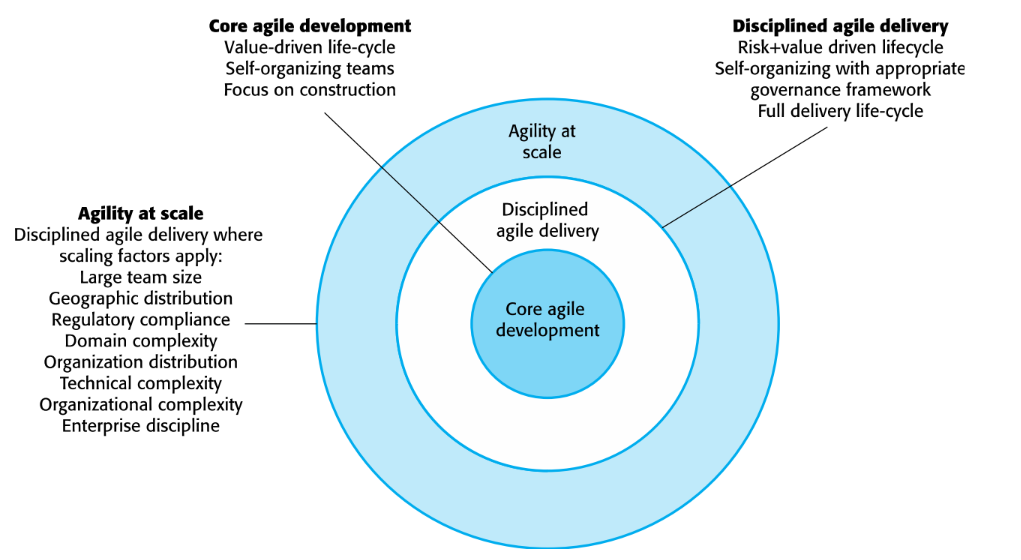
\includegraphics[width=0.6\linewidth]{images/ibm-agility-scale-model.PNG}
    \caption{Modello agile di IBM}
    \label{fig:ibm-agility-scale-model}
\end{figure}

Non esiste un modello unico adatto a tutti i prodotti agili su larga scala, poiché il tipo di prodotto, i requisiti del cliente e le persone disponibili sono tutti diversi. Tuttavia, gli approcci per scalare i metodi agili hanno una serie di punti in comune:
\begin{enumerate}
    \item Impossibilità di un approccio completamente incrementale all'ingegneria dei requisiti.
    \item Non può esserci un unico proprietario del prodotto o rappresentante del cliente. 
    \item Non è possibile concentrarsi solo sul codice del sistema. 
    \item Devono essere progettati e utilizzati meccanismi di comunicazione tra i team.
    \item Mantenere un'integrazione continua. Tuttavia, è essenziale mantenere costruzioni frequenti del sistema e rilasci regolari del sistema.
\end{enumerate}
Scrum è stato adattato per lo sviluppo su larga scala. Le caratteristiche chiave dello Scrum multi-team sono:
\begin{enumerate}
    \item \textit{Replica dei ruoli:} Ogni team ha un Product Owner per la propria componente di lavoro e un ScrumMaster.
    \item \textit{Architetti del prodotto:} Ogni team sceglie un architetto del prodotto, e questi architetti collaborano per progettare e far evolvere l'architettura complessiva del sistema.
    \item \textit{Allineamento delle versioni:} Le date delle versioni del prodotto di ciascun team sono allineate in modo da produrre un sistema dimostrabile e completo.
    \item \textit{Scrum of Scrums:} C'è uno Scrum of Scrums quotidiano in cui i rappresentanti di ciascun team si incontrano per discutere i progressi, identificare problemi e pianificare il lavoro da svolgere quel giorno.
\end{enumerate}

\subsection{Metodi agili nelle organizzazioni}
Può essere difficile introdurre metodi agili in grandi aziende per diversi motivi:
\begin{enumerate}
    \item I project manager che non hanno esperienza con i metodi agili possono essere riluttanti ad accettare il rischio di un nuovo approccio.
    \item Le grandi organizzazioni spesso hanno procedure e standard di qualità che tutti i progetti sono tenuti a seguire e, a causa della loro natura burocratica, è probabile che questi siano incompatibili con i metodi agili.
    \item I metodi agili sembrano funzionare meglio quando i membri del team hanno un livello di abilità relativamente alto. Tuttavia, all'interno delle grandi organizzazioni, è probabile che ci sia una vasta gamma di competenze e abilità.
    \item Potrebbe esserci una resistenza culturale ai metodi agili, specialmente in quelle organizzazioni che hanno una lunga storia nell'uso di processi ingegneristici convenzionali.
\end{enumerate}

\section{Punti chiave}
\begin{center}
\begin{minipage}{\textwidth}
\colorbox{lightgray}{
\parbox{\linewidth}{
\begin{itemize} 
    \item I metodi agili sono metodi di sviluppo incrementali che si concentrano sullo sviluppo rapido del software, sulle frequenti release del software, sulla riduzione delle spese generali dei processi riducendo al minimo la documentazione e sulla produzione di codice di alta qualità.
    \item Le pratiche di sviluppo agile includono requisiti espressi come Storie utente per le specifiche di sistema, rilasci frequenti del software, miglioramento continuo del software, sviluppo test-first e partecipazione del cliente al team di sviluppo.
    \item Scrum è un metodo agile che fornisce un framework per organizzare progetti agili. È incentrato su un insieme di sprint, che sono periodi di tempo fissi in cui viene sviluppato un incremento del sistema.
    \item Molti metodi di sviluppo pratici sono un mix di sviluppo agile e plan-driven.
    \item È difficile adattare i metodi agili ai sistemi di grandi dimensioni. I sistemi di grandi dimensioni necessitano di una progettazione iniziale e di una certa documentazione e le pratiche organizzative possono entrare in conflitto con l'informalità degli approcci agili.
\end{itemize}
}}
\end{minipage}
\end{center}